\section{Latent and Low-Rank Attention Families}
\label{sec:annex-latent}

This annex covers the latent / low-rank KV compression family of attention mechanisms. These architectures compress the per-token key--value state into a low-rank latent vector that is the only quantity materialised in the KV cache during decoding, then reconstruct full multi-head keys and values on the fly. The family unifies grouped-query, latent, factorised, and temporal-latent designs under a common low-rank bottleneck.

\subsection{Multi-Head Latent Attention (MLA)}

\begin{figure}[H]
\centering
\fitfigure{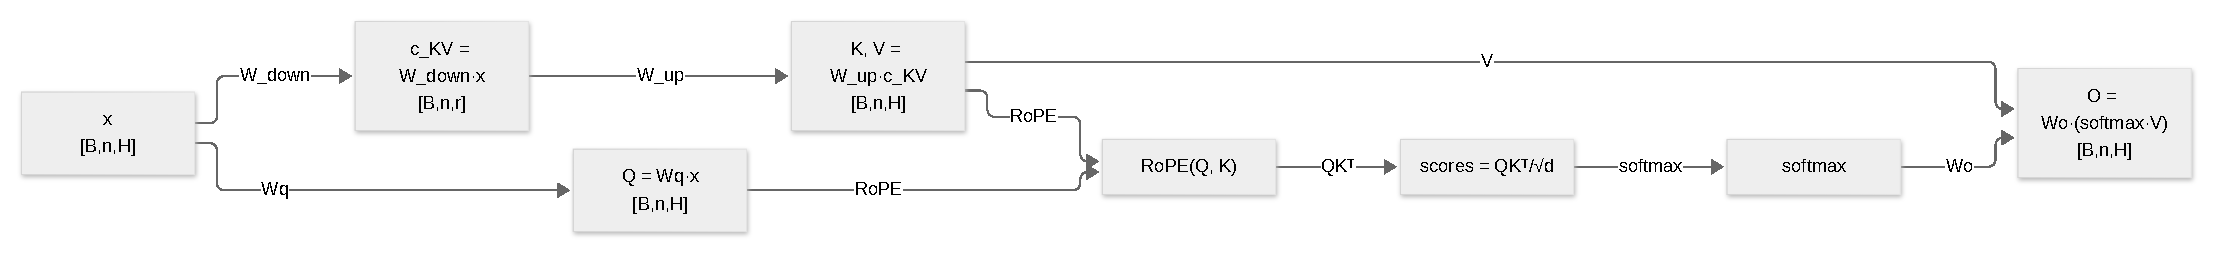
\includegraphics{figures/mixers/mla.pdf}}
\caption{Dataflow of multi-head latent attention: keys and values are down-projected to a low-rank latent, up-projected back, and attended with the query after RoPE.}
\label{fig:mixer-mla}
\end{figure}
Multi-Head Latent Attention (MLA) \citep{mehta_mla_2025} compresses the per-token key--value state into a single low-rank latent vector $c_{KV}$ of rank $r_{kv}$, which is the only quantity materialised in the KV cache during decoding. A pair of up-projection matrices reconstructs the full multi-head keys and values on the fly, while RoPE is applied to the decompressed query and key tensors so that positional structure is preserved. The authors show that the Pareto-optimal latent width sits near $r_{kv} = d_{\text{hidden}} / 2$, at which point MLA halves the KV cache yet matches multi-head attention (MHA) quality on small models.

\subsubsection{Mathematical Formulation}
\[
c_{KV} = W_{DKV}\, x \in \mathbb{R}^{r_{kv}}, \qquad
k = W_{UK}\, c_{KV}, \qquad
v = W_{UV}\, c_{KV}, \qquad
q = W_{Q}\, x.
\]
\[
\tilde q = \text{RoPE}(q), \quad \tilde k = \text{RoPE}(k), \qquad
\text{attn} = \texttt{softmax}\!\left(\frac{\tilde q\, \tilde k^\top}{\sqrt{d_h}}\right) v.
\]

\subsubsection{Algorithmic Pseudocode}
\begin{algorithmic}[1]
\State \textbf{Input:} hidden state $x \in \mathbb{R}^{n \times d}$, rank $r_{kv}$, projections $W_{DKV}, W_{UK}, W_{UV}, W_{Q}$
\State $c_{KV} \gets W_{DKV}\, x$ \Comment{down-project to latent of rank $r_{kv}$ (cached at inference)}
\State $k \gets W_{UK}\, c_{KV}$, \quad $v \gets W_{UV}\, c_{KV}$ \Comment{up-project to full heads}
\State $q \gets W_{Q}\, x$
\State $\tilde q \gets \text{RoPE}(q)$, \quad $\tilde k \gets \text{RoPE}(k)$ \Comment{apply rotary embeddings}
\State $\text{weights} \gets \texttt{softmax}(\tilde q\, \tilde k^\top / \sqrt{d_h})$
\State \textbf{Output:} $\mathbf{Y} = \text{weights} \cdot v$
\end{algorithmic}

\subsubsection{Key Characteristics}
\begin{itemize}[leftmargin=*]
    \item \textbf{Training complexity}: $\mathcal{O}(n^2 \cdot d)$ (full attention on decompressed heads).
    \item \textbf{Inference complexity}: $\mathcal{O}(n)$ per token, $\mathcal{O}(r_{kv} \cdot n)$ KV-cache space (latent only).
    \item \textbf{Trainable}: fully trainable; $r_{kv}$ is a hyperparameter (Pareto-optimal $\approx d/2$).
    \item \textbf{Strengths}: Halves KV cache versus MHA at matched quality; RoPE-compatible; clean latent bottleneck.
    \item \textbf{Limitations}: Up-projection adds decode FLOPs; latent rank is a fixed global budget shared across heads.
\end{itemize}

\subsection{Group-Query Latent Attention (GQLA)}

\begin{figure}[H]
\centering
\fitfigure{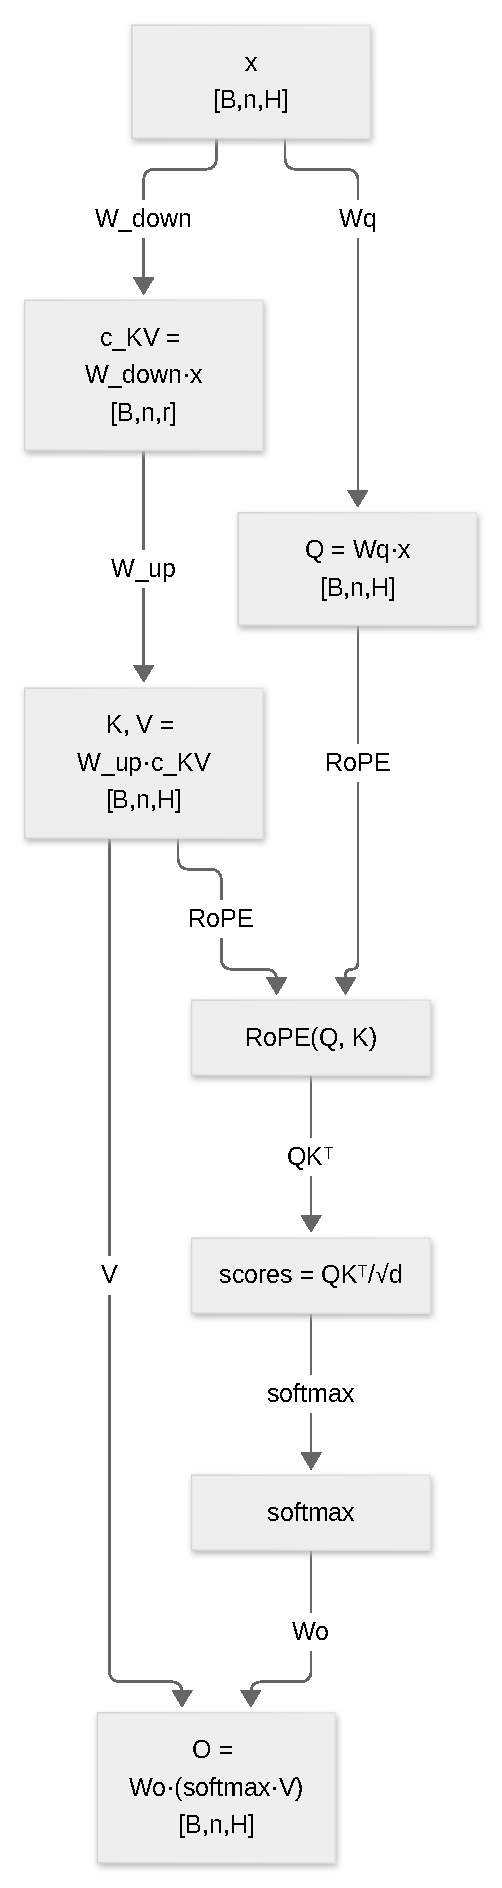
\includegraphics{figures/mixers/gqla.pdf}}
\caption{Dataflow of group-query latent attention: the shared latent cache is up-projected to key/value heads and combined with grouped queries.}
\label{fig:mixer-gqla}
\end{figure}
Group-Query Latent Attention (GQLA) \citep{meng_gqla_2026} is a minimal modification of MLA that exposes two algebraically equivalent decoding paths over the same trained weights: an MQA-absorb path (fusing the up-projection into the query, optimal on H100-class hardware) and a GQA-expanded path (materialising full keys/values, optimal on H20 / multi-token-prediction hardware). The two paths are mathematically identical because the up-projection is linear, so $\texttt{softmax}(q_{\text{absorbed}} \cdot c_{KV}^\top) = \texttt{softmax}((q \cdot W_{UK}^\top) \cdot c_{KV}^\top)$, allowing hardware-adaptive dispatch with no retraining.

\subsubsection{Mathematical Formulation}
Same latent as MLA:
\[
c_{KV} = W_{DKV}\, x, \qquad k = W_{UK}\, c_{KV}, \qquad v = W_{UV}\, c_{KV}, \qquad q = W_{Q}\, x.
\]
\[
\text{Path A (MQA-absorb): } \text{attn} = \texttt{softmax}\!\left(\frac{(q\, W_{UK}^\top)\, c_{KV}^\top}{\sqrt{d_h}}\right) (W_{UV}\, c_{KV}).
\]
\[
\text{Path B (GQA-expanded): } \text{attn} = \texttt{softmax}\!\left(\frac{q\, k^\top}{\sqrt{d_h}}\right) v, \quad k = W_{UK} c_{KV},\ v = W_{UV} c_{KV}.
\]

\subsubsection{Algorithmic Pseudocode}
\begin{algorithmic}[1]
\State \textbf{Input:} $x$, weights $W_{DKV}, W_{UK}, W_{UV}, W_{Q}$, hardware flag $\text{hw} \in \{\text{H100}, \text{H20}\}$
\State $c_{KV} \gets W_{DKV}\, x$ \Comment{shared latent, cached}
\State $q \gets W_{Q}\, x$
\If{$\text{hw} == \text{H100}$} \Comment{MQA-absorb path}
    \State $q_{\text{abs}} \gets q\, W_{UK}^\top$ \Comment{absorb up-projection into query}
    \State $\text{weights} \gets \texttt{softmax}(q_{\text{abs}}\, c_{KV}^\top / \sqrt{d_h})$
    \State $\mathbf{Y} \gets \text{weights} \cdot (W_{UV}\, c_{KV})$
\Else \Comment{GQA-expanded path}
    \State $k \gets W_{UK}\, c_{KV}$, \quad $v \gets W_{UV}\, c_{KV}$
    \State $\text{weights} \gets \texttt{softmax}(q\, k^\top / \sqrt{d_h})$
    \State $\mathbf{Y} \gets \text{weights} \cdot v$
\EndIf
\State \textbf{Output:} $\mathbf{Y}$
\end{algorithmic}

\subsubsection{Key Characteristics}
\begin{itemize}[leftmargin=*]
    \item \textbf{Training complexity}: $\mathcal{O}(n^2 \cdot d)$, identical to MLA.
    \item \textbf{Inference complexity}: $\mathcal{O}(n)$ per token, $\mathcal{O}(r_{kv} \cdot n)$ latent state; path chosen by hardware.
    \item \textbf{Trainable}: trained once; the two decoding paths reuse the same weights.
    \item \textbf{Strengths}: Hardware-adaptive decode with no quality loss; algebraic equivalence guarantees consistency.
    \item \textbf{Limitations}: Same latent-rank tradeoffs as MLA; path selection is a deployment-time heuristic.
\end{itemize}

\subsection{Multi-Head Low-Rank Attention (MLRA)}

\begin{figure}[H]
\centering
\fitfigure{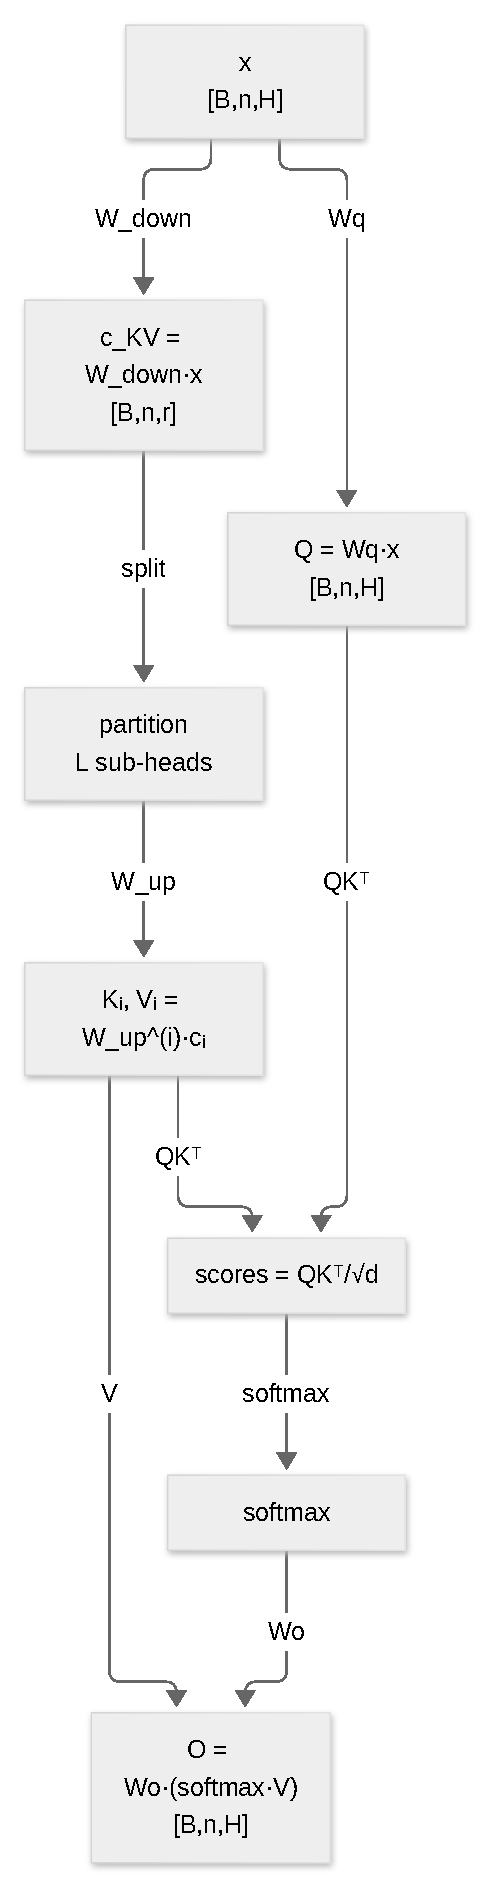
\includegraphics{figures/mixers/mlra.pdf}}
\caption{Dataflow of multi-head low-rank attention: the latent is partitioned across sub-heads, each with its own up-projection, before attention.}
\label{fig:mixer-mlra}
\end{figure}
Multi-Head Low-Rank Attention (MLRA) \citep{liu_mlra_2026} refactors the single MLA latent into $L$ disjoint sub-heads each of rank $r/L$, so that the KV cache can be partitioned across $L$ devices for 4-way tensor-parallel decoding (each device loads only $1/L$ of the cache). Per-sub-head up-projections reconstruct the corresponding slice of the full heads and are concatenated, yielding a 2.8$\times$ decode speedup over MLA while preserving the global latent budget.

\subsubsection{Mathematical Formulation}
\[
c_{KV} = [c_1, c_2, \ldots, c_L], \quad c_i \in \mathbb{R}^{r/L}, \qquad c_{KV} = W_{DKV}\, x.
\]
\[
k_i = W_{UK}^{(i)}\, c_i, \quad v_i = W_{UV}^{(i)}\, c_i, \qquad
k = [k_1; \ldots; k_L], \quad v = [v_1; \ldots; v_L].
\]
\[
\text{attn} = \texttt{softmax}\!\left(\frac{q\, k^\top}{\sqrt{d_h}}\right) v.
\]

\subsubsection{Algorithmic Pseudocode}
\begin{algorithmic}[1]
\State \textbf{Input:} $x$, sub-head count $L$, per-sub-head projections $W_{UK}^{(i)}, W_{UV}^{(i)}$
\State $c_{KV} \gets W_{DKV}\, x = [c_1, \ldots, c_L]$ \Comment{partition latent into $L$ blocks}
\For{$i = 1, \ldots, L$ (parallel across $L$ devices)}
    \State $k_i \gets W_{UK}^{(i)}\, c_i$, \quad $v_i \gets W_{UV}^{(i)}\, c_i$
\EndFor
\State $k \gets \texttt{concat}(k_1, \ldots, k_L)$, \quad $v \gets \texttt{concat}(v_1, \ldots, v_L)$
\State $\text{weights} \gets \texttt{softmax}(q\, k^\top / \sqrt{d_h})$
\State \textbf{Output:} $\mathbf{Y} = \text{weights} \cdot v$
\end{algorithmic}

\subsubsection{Key Characteristics}
\begin{itemize}[leftmargin=*]
    \item \textbf{Training complexity}: $\mathcal{O}(n^2 \cdot d)$ (full attention on concatenated heads).
    \item \textbf{Inference complexity}: $\mathcal{O}(n)$ per token, $\mathcal{O}(r_{kv} \cdot n)$ state partitioned across $L$ devices.
    \item \textbf{Trainable}: fully trainable; $L$ controls partition granularity.
    \item \textbf{Strengths}: 2.8$\times$ decode speedup; clean 4-way tensor-parallel cache sharding; preserves total latent budget.
    \item \textbf{Limitations}: Requires $L$ to divide $r_{kv}$; more projection matrices than MLA; inter-device all-reduce on output.
\end{itemize}

\subsection{Tucker Attention}

\begin{figure}[H]
\centering
\fitfigure{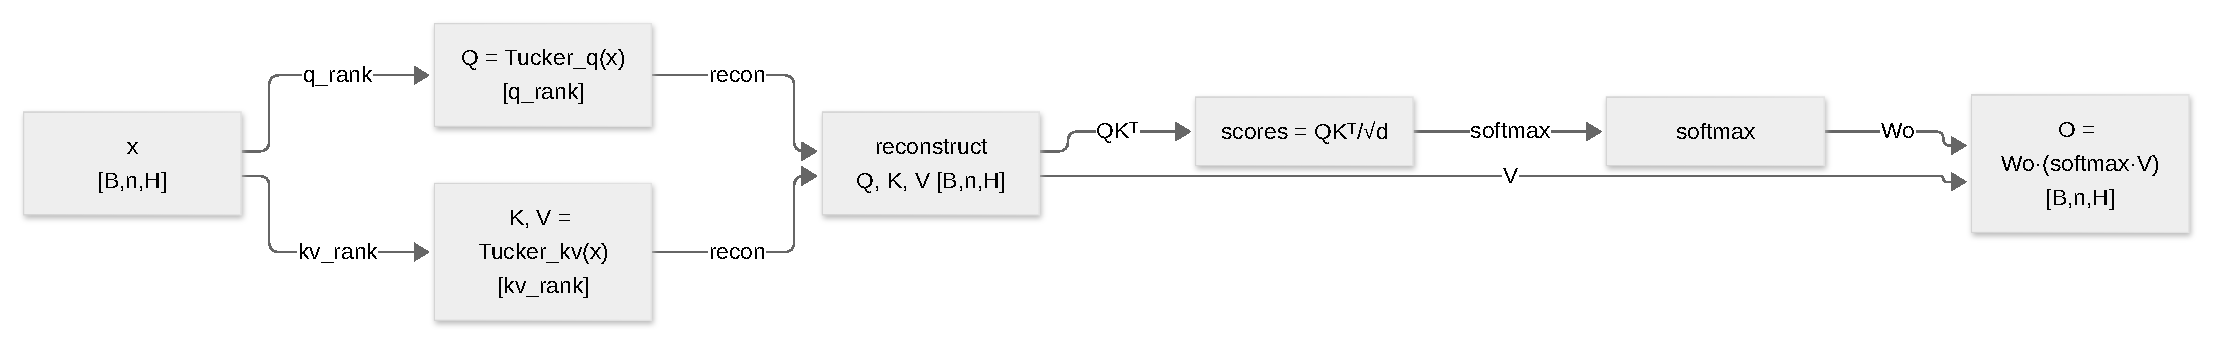
\includegraphics{figures/mixers/tucker.pdf}}
\caption{Dataflow of Tucker attention: queries and key/values are projected through Tucker factors and reconstructed before the scaled dot product.}
\label{fig:mixer-tucker}
\end{figure}
Tucker Attention \citep{klein_tucker_2026} unifies MHA, GQA and MLA under a single Tucker-style factorisation of the query/key/value weight tensors with independent ranks $q_{\text{rank}}, k_{\text{rank}}, v_{\text{rank}}$. MHA is recovered when all ranks equal the hidden size, GQA when $k_{\text{rank}} = v_{\text{rank}} < d$, and MLA when $k_{\text{rank}} = v_{\text{rank}}$ equals the latent rank. Because the factorisation is a pure linear reparameterisation, the method is fully compatible with FlashAttention and RoPE, and yields an order of magnitude fewer parameters for comparable metrics.

\subsubsection{Mathematical Formulation}
\[
\mathbf{Q} = W_{Q,\text{core}}\, W_{Q,\text{factor}}\, x, \qquad
\mathbf{K} = W_{K,\text{core}}\, W_{K,\text{factor}}\, x, \qquad
\mathbf{V} = W_{V,\text{core}}\, W_{V,\text{factor}}\, x.
\]
\[
\text{attn} = \texttt{softmax}\!\left(\frac{\mathbf{Q}\, \mathbf{K}^\top}{\sqrt{d_h}}\right) \mathbf{V}.
\]
Special cases: MHA $\Leftrightarrow q_{\text{rank}} = k_{\text{rank}} = v_{\text{rank}} = d$; GQA $\Leftrightarrow k_{\text{rank}} = v_{\text{rank}} < d$; MLA $\Leftrightarrow k_{\text{rank}} = v_{\text{rank}} = r_{kv}$.

\subsubsection{Algorithmic Pseudocode}
\begin{algorithmic}[1]
\State \textbf{Input:} $x$, ranks $q_{\text{rank}}, k_{\text{rank}}, v_{\text{rank}}$, core/factor matrices
\State $\mathbf{Q} \gets W_{Q,\text{core}}\, W_{Q,\text{factor}}\, x$ \Comment{rank-$q_{\text{rank}}$ factorised query}
\State $\mathbf{K} \gets W_{K,\text{core}}\, W_{K,\text{factor}}\, x$ \Comment{rank-$k_{\text{rank}}$ factorised key}
\State $\mathbf{V} \gets W_{V,\text{core}}\, W_{V,\text{factor}}\, x$ \Comment{rank-$v_{\text{rank}}$ factorised value}
\State \textbf{Apply RoPE to $\mathbf{Q}, \mathbf{K}$ if positional encoding is used}
\State $\text{weights} \gets \texttt{softmax}(\mathbf{Q}\, \mathbf{K}^\top / \sqrt{d_h})$ \Comment{FlashAttention-compatible}
\State \textbf{Output:} $\mathbf{Y} = \text{weights} \cdot \mathbf{V}$
\end{algorithmic}

\subsubsection{Key Characteristics}
\begin{itemize}[leftmargin=*]
    \item \textbf{Training complexity}: $\mathcal{O}(n^2 \cdot d)$ on the reconstructed tensors.
    \item \textbf{Inference complexity}: $\mathcal{O}(n)$ per token; cache size governed by $k_{\text{rank}}$.
    \item \textbf{Trainable}: ranks are hyperparameters; the factorisation is a drop-in weight reparameterisation.
    \item \textbf{Strengths}: Unifies MHA/GQA/MLA; order-of-magnitude parameter reduction at matched metrics; FlashAttention/RoPE compatible.
    \item \textbf{Limitations}: Two matmuls per projection add latency; rank selection is a per-task tuning problem.
\end{itemize}

\subsection{Interleaved Head Attention (IHA)}

\begin{figure}[H]
\centering
\fitfigure{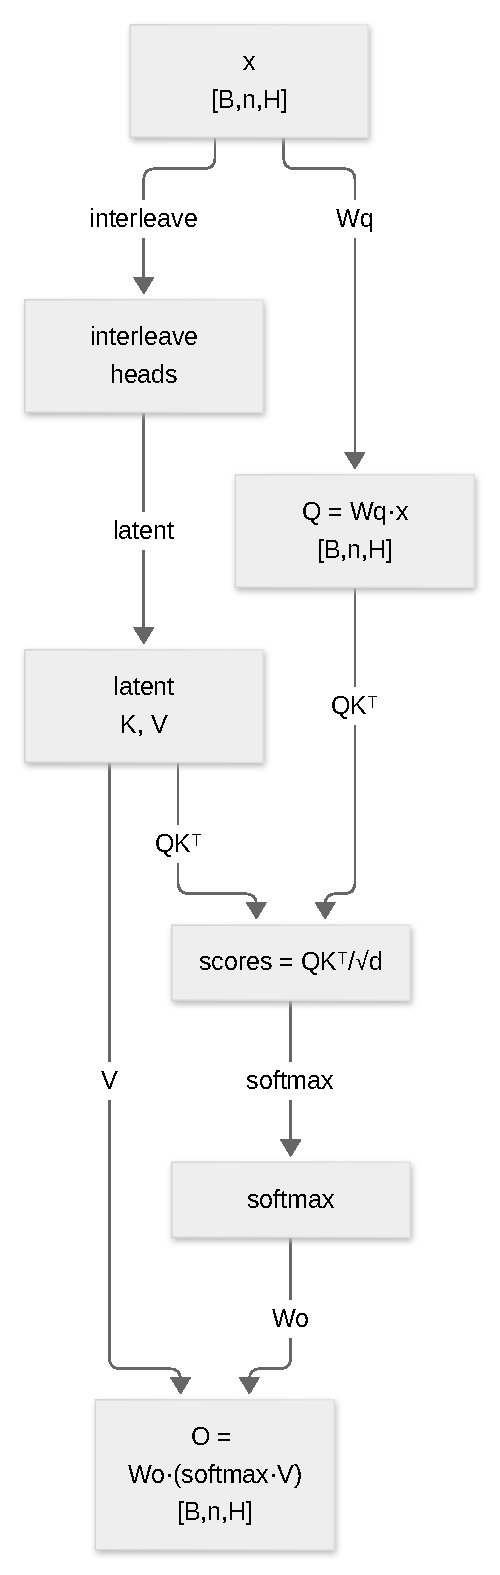
\includegraphics{figures/mixers/iha.pdf}}
\caption{Dataflow of interleaved-head attention: heads are interleaved into a latent key/value representation that is attended by the query.}
\label{fig:mixer-iha}
\end{figure}
Interleaved Head Attention (IHA) \citep{duvvuri_iha_2026} constructs $P$ pseudo-heads per original head (typically $P = H$) where each pseudo query/key/value is a learned linear combination of all $H$ original heads. This induces up to $P^2$ distinct attention patterns per head at an $\mathcal{O}(H^2 P)$ overhead. Theoretically, IHA needs only $\Theta(\sqrt{k}\, n^2)$ parameters versus $\Theta(k\, n^2)$ for MHA on the Polynomial task; empirically it delivers $+10$--$20\%$ on RULER multi-key retrieval, $+5.8\%$ on GSM8K and $+2.8\%$ on MATH-500.

\subsubsection{Mathematical Formulation}
{\small
\[
q_{\text{pseudo}}[p] = \sum_{h=1}^{H} \text{mix}_q[p, h]\, q[h], \quad
k_{\text{pseudo}}[p] = \sum_{h} \text{mix}_k[p, h]\, k[h], \quad
v_{\text{pseudo}}[p] = \sum_{h} \text{mix}_v[p, h]\, v[h].
\]
}
\[
\text{attn}_p = \texttt{softmax}\!\left(\frac{q_{\text{pseudo}}[p]\, k_{\text{pseudo}}[p]^\top}{\sqrt{d_h}}\right) v_{\text{pseudo}}[p],
\qquad
\mathbf{Y}[h] = \frac{1}{P} \sum_{p} \text{attn}_p[h].
\]

\subsubsection{Algorithmic Pseudocode}
\begin{algorithmic}[1]
\State \textbf{Input:} per-head $q[h], k[h], v[h]$, mixing matrices $\text{mix}_q, \text{mix}_k, \text{mix}_v \in \mathbb{R}^{P \times H}$
\For{$p = 1, \ldots, P$}
    \State $q_p \gets \sum_h \text{mix}_q[p,h]\, q[h]$ \Comment{learned mix across heads}
    \State $k_p \gets \sum_h \text{mix}_k[p,h]\, k[h]$, \quad $v_p \gets \sum_h \text{mix}_v[p,h]\, v[h]$
    \State $\text{attn}_p \gets \texttt{softmax}(q_p\, k_p^\top / \sqrt{d_h})\, v_p$
\EndFor
\State \textbf{Output:} $\mathbf{Y}[h] \gets \frac{1}{P} \sum_p \text{attn}_p[h]$ \Comment{average pseudo-head outputs per head}
\end{algorithmic}

\subsubsection{Key Characteristics}
\begin{itemize}[leftmargin=*]
    \item \textbf{Training complexity}: $\mathcal{O}(n^2 \cdot H \cdot P)$ with $P \approx H$, i.e.\ $\mathcal{O}(n^2 \cdot H^2)$.
    \item \textbf{Inference complexity}: $\mathcal{O}(n)$ per token with KV cache; extra $\mathcal{O}(H^2 P)$ mixing overhead.
    \item \textbf{Trainable}: mixing matrices are learned; $P$ is a hyperparameter.
    \item \textbf{Strengths}: $\Theta(\sqrt{k})$ parameter efficiency on Polynomial; large gains on retrieval and reasoning benchmarks.
    \item \textbf{Limitations}: Quadratic-in-heads mixing cost; more attention patterns to compute; added latency at large $H$.
\end{itemize}

\subsection{Grouped-head laTenT Attention (GTA)}

\begin{figure}[H]
\centering
\fitfigure{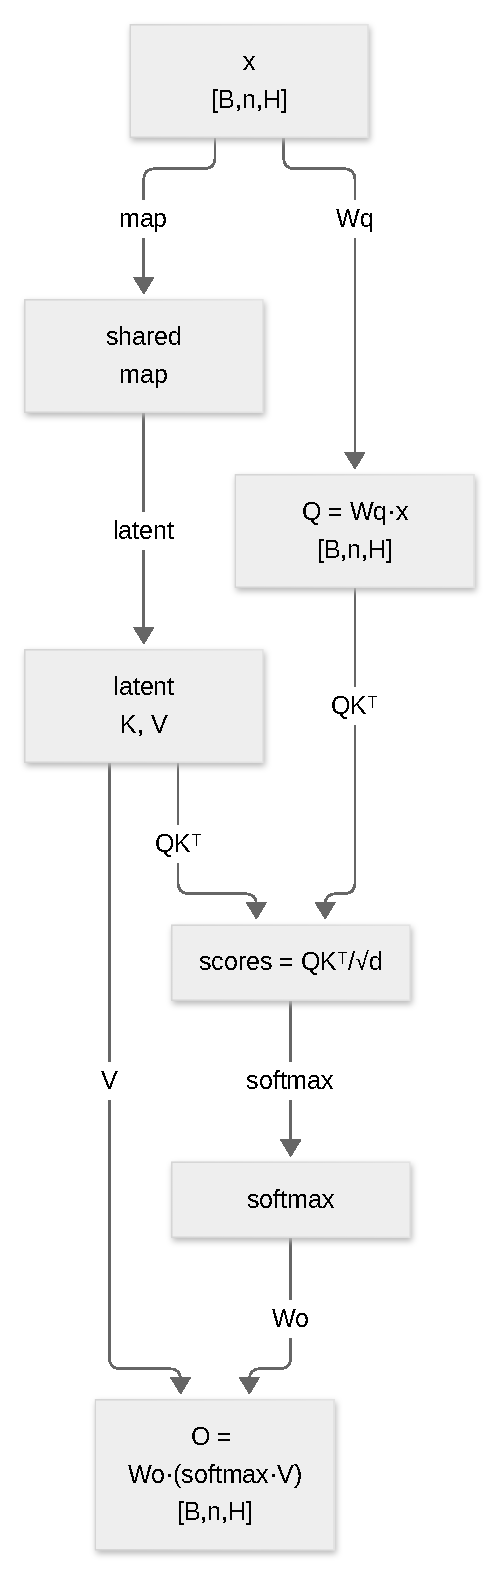
\includegraphics{figures/mixers/gta.pdf}}
\caption{Dataflow of grouped-head latent attention: a shared map produces the latent key/value state consumed by the grouped heads.}
\label{fig:mixer-gta}
\end{figure}
Grouped-head laTenT Attention (GTA) \citep{sun_gta_2025} combines two compressions: (1) a \emph{shared attention map} --- one attention-score tensor per group of heads, reused across all heads in the group, shrinking the key cache; and (2) a \emph{nonlinear value decoder} --- the value cache is compressed to a latent by a down-projection and reconstructed by a SiLU-gated up-projection before the output projection. GTA cuts attention FLOPs by up to 62.5\% versus GQA, shrinks the KV cache by up to 70\%, and yields a 2$\times$ end-to-end inference speedup.

\subsubsection{Mathematical Formulation}
{\footnotesize
\[
q_g = \texttt{mean}(q[\text{group } g]), \quad k_g = \texttt{mean}(k[\text{group } g]), \quad
\text{attn}_g = \texttt{softmax}\!\left(\frac{q_g\, k_g^\top}{\sqrt{d_h}}\right) \text{ (reused across the group)}.
\]
}
\[
v_{\text{latent}} = W_{DV}\, x, \qquad v = \text{SiLU}(W_{UV}\, v_{\text{latent}}), \qquad
\mathbf{Y} = \text{attn}_g \cdot v.
\]

\subsubsection{Algorithmic Pseudocode}
\begin{algorithmic}[1]
\State \textbf{Input:} $q, k$ per head, hidden $x$, group partition $\{g\}$
\State $v_{\text{latent}} \gets W_{DV}\, x$ \Comment{compress values to latent (cached)}
\State $v \gets \text{SiLU}(W_{UV}\, v_{\text{latent}})$ \Comment{nonlinear value decode}
\For{each group $g$}
    \State $q_g \gets \texttt{mean}(q[g])$, \quad $k_g \gets \texttt{mean}(k[g])$ \Comment{shared per-group queries/keys}
    \State $\text{attn}_g \gets \texttt{softmax}(q_g\, k_g^\top / \sqrt{d_h})$
    \State $\mathbf{Y}[g] \gets \text{attn}_g \cdot v[g]$ \Comment{one map reused for all heads in $g$}
\EndFor
\State \textbf{Output:} $\mathbf{Y}$
\end{algorithmic}

\subsubsection{Key Characteristics}
\begin{itemize}[leftmargin=*]
    \item \textbf{Training complexity}: $\mathcal{O}(n^2 \cdot G \cdot d_h)$ where $G$ is the number of groups (vs $H$ heads for GQA).
    \item \textbf{Inference complexity}: $\mathcal{O}(n)$ per token; value cache $\mathcal{O}(r_v \cdot n)$, key cache reduced by group sharing.
    \item \textbf{Trainable}: group assignment and latent rank are trainable/hyperparameters.
    \item \textbf{Strengths}: up to 62.5\% attention-FLOP reduction, 70\% KV-cache shrink, 2$\times$ end-to-end speedup.
    \item \textbf{Limitations}: Shared map reduces per-head diversity; nonlinear decoder adds latency; grouping must be chosen carefully.
\end{itemize}

\subsection{Multi-head Temporal Latent Attention (MTLA)}

\begin{figure}[H]
\centering
\fitfigure{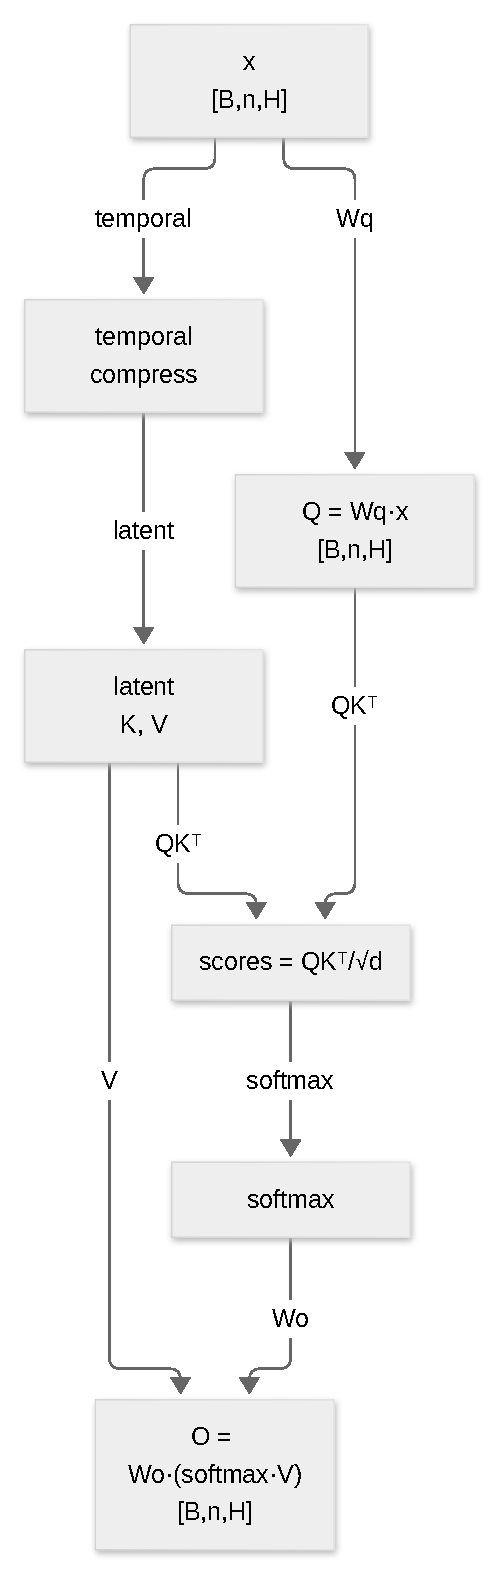
\includegraphics{figures/mixers/mtla.pdf}}
\caption{Dataflow of multi-head temporal latent attention: a temporal compression stage produces the latent key/value state attended by the query.}
\label{fig:mixer-mtla}
\end{figure}
Multi-head Temporal Latent Attention (MTLA) \citep{deng_mtla_2025} extends MLA along the temporal axis: a hyper-network dynamically merges $m$ temporally adjacent KV-cache vectors into a single slot, shrinking the temporal length by a factor of $m$. A stride-aware causal mask keeps parallel training consistent with autoregressive inference, yielding a 5.3$\times$ decode speedup and 8.3$\times$ GPU-memory reduction versus MHA on En--De speech translation.

\subsubsection{Mathematical Formulation}
\[
c_{KV}^{(t)} = W_{DKV}\, x^{(t)} \in \mathbb{R}^{r_{kv}} \text{ (per-token latent)}.
\]
\[
\bar c_{KV}^{(j)} = \sum_{i=0}^{m-1} \alpha_i\, c_{KV}^{(s j + i)}, \qquad \alpha_i = \texttt{sigmoid}(\text{HyperNet}(c_{KV}^{(s j + i)})),
\]
where $s$ is the stride and $m$ the merge window. Queries attend over merged slots $\bar c_{KV}$ with a stride-aware causal mask $M_{\text{stride}}$:
\[
\text{attn} = \texttt{softmax}\!\left(\frac{q\, \bar k^\top}{\sqrt{d_h}} + M_{\text{stride}}\right) \bar v, \quad \bar k = W_{UK}\, \bar c_{KV},\ \bar v = W_{UV}\, \bar c_{KV}.
\]

\subsubsection{Algorithmic Pseudocode}
\begin{algorithmic}[1]
\State \textbf{Input:} per-token latents $c_{KV}^{(t)}$, merge window $m$, stride $s$
\State \textbf{Merge phase (hyper-network):}
\For{each merged slot $j = 0, 1, \ldots$}
    \State $\alpha_i \gets \texttt{sigmoid}(\text{HyperNet}(c_{KV}^{(s j + i)}))$ for $i = 0, \ldots, m-1$
    \State $\bar c_{KV}^{(j)} \gets \sum_{i=0}^{m-1} \alpha_i\, c_{KV}^{(s j + i)}$ \Comment{gated average over window}
\EndFor
\State $\bar k \gets W_{UK}\, \bar c_{KV}$, \quad $\bar v \gets W_{UV}\, \bar c_{KV}$
\State $\text{weights} \gets \texttt{softmax}(q\, \bar k^\top / \sqrt{d_h} + M_{\text{stride}})$ \Comment{stride-aware causal mask}
\State \textbf{Output:} $\mathbf{Y} = \text{weights} \cdot \bar v$
\end{algorithmic}

\subsubsection{Key Characteristics}
\begin{itemize}[leftmargin=*]
    \item \textbf{Training complexity}: $\mathcal{O}(n^2 \cdot d / m)$ on the merged sequence (length $\lceil n/m \rceil$) plus hyper-network cost.
    \item \textbf{Inference complexity}: $\mathcal{O}(n/m)$ per token over merged slots; $\mathcal{O}(r_{kv} \cdot n / m)$ state.
    \item \textbf{Trainable}: hyper-network and merge window $m$ are learned/chosen; stride-aware mask enforces consistency.
    \item \textbf{Strengths}: 5.3$\times$ decode speedup, 8.3$\times$ GPU-memory reduction vs MHA; temporal compression orthogonal to rank compression.
    \item \textbf{Limitations}: Merge window can blur fine temporal detail; hyper-network adds compute; mask design is non-trivial.
\end{itemize}

\subsection{Architectural Comparison and Synthesis}

\subsection{Compressed Convolutional Attention (CCA)}

\begin{figure}[H]
\centering
\fitfigure{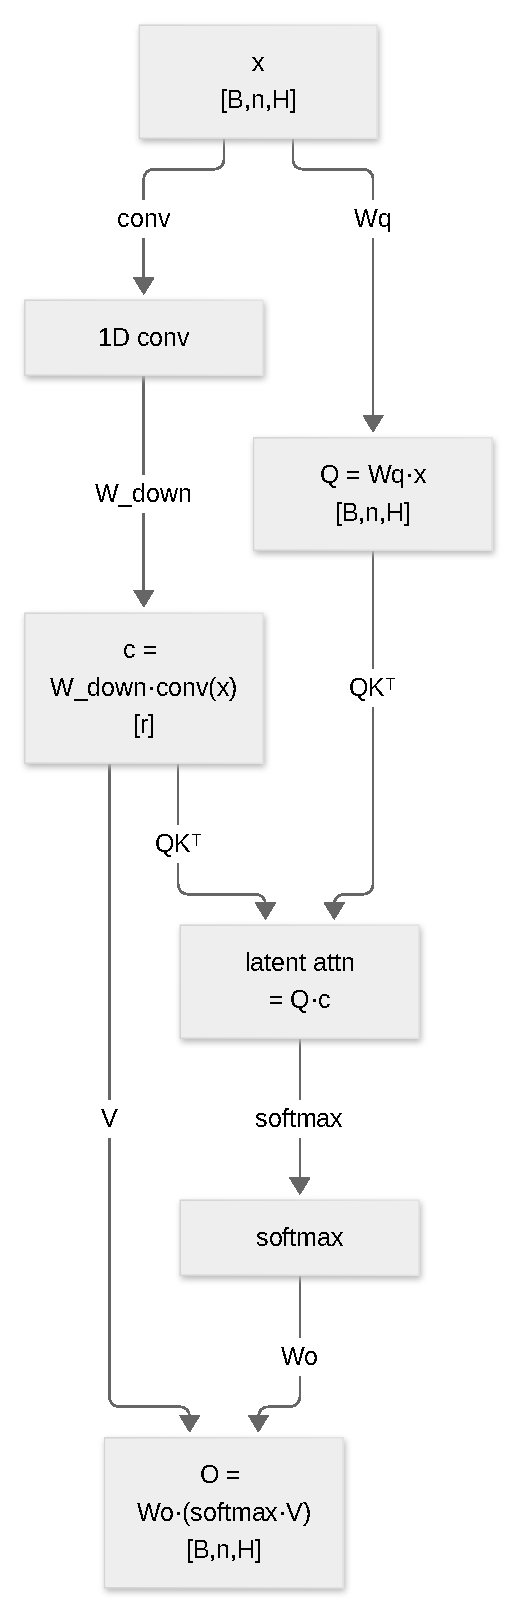
\includegraphics{figures/mixers/cca.pdf}}
\caption{Dataflow of compressed convolutional attention: a 1D convolution feeds a latent compression $c$, which the query attends directly.}
\label{fig:mixer-cca}
\end{figure}
Compressed Convolutional Attention (CCA) \citep{figliola_cca_2025} takes a fundamentally different approach to latent attention: rather than compressing the KV-cache and then up-projecting to full width before attending (as MLA/GQLA/MLRA do), CCA down-projects queries, keys, and values into a shared latent and performs the \emph{entire} attention operation inside it. There are no Q/K/V up-projection matrices---only a single output up-projection $\tilde{W}_O$ maps the latent output back to the residual stream. This simultaneously reduces parameters, KV-cache size, \textbf{and} attention FLOPs by the compression factor $C = E/\tilde{e}$, whereas MLA only shrinks the cache.

To make attention in the fully compressed latent viable, CCA introduces three innovations: (1) two causal convolutions on the packed q/k tensor (a depth-wise sequence convolution and a head-wise grouped channel convolution), (2) q-k-mean (adds the pre-convolution mean of q and k to the post-convolution values), and (3) value-shift (each head receives half its values from the current token and half from the previous token via two independent projections). After these steps, QK L2-normalisation and a learnable key temperature $\beta$ are applied, RoPE is applied \emph{directly in the latent} (no separate RoPE head needed), and standard softmax attention is computed.

\subsubsection{Mathematical Formulation}
\[
\tilde{q}_{\text{pre}} = \tilde{W}_Q\, x, \qquad \tilde{k}_{\text{pre}} = \tilde{W}_K\, x, \qquad \tilde{e} = E / C.
\]
\[
\tilde{q} = \text{Conv}(\tilde{q}_{\text{pre}}) + \tfrac{1}{2}(\tilde{q}_{\text{pre}} + \tilde{k}_{\text{pre}}), \qquad
\tilde{k} = \text{Conv}(\tilde{k}_{\text{pre}}) + \tfrac{1}{2}(\tilde{q}_{\text{pre}} + \tilde{k}_{\text{pre}}).
\]
\[
\tilde{v} = [\tilde{W}_{V_1}\, x_t \;\|\; \tilde{W}_{V_2}\, x_{t-1}], \qquad
\hat{q} = \frac{\tilde{q} \sqrt{d_h}}{\|\tilde{q}\|}, \quad \hat{k} = \frac{\tilde{k} \sqrt{d_h}}{\|\tilde{k}\|} e^{\beta}.
\]
\[
\text{attn} = \texttt{softmax}\!\left(\frac{\text{RoPE}(\hat{q})\, \text{RoPE}(\hat{k})^\top}{\sqrt{d_h}}\right) \tilde{v}, \qquad
\mathbf{Y} = \tilde{W}_O\, \text{attn}.
\]

\subsubsection{Algorithmic Pseudocode}
\begin{algorithmic}[1]
\State \textbf{Input:} hidden state $x \in \mathbb{R}^{n \times E}$, compression factor $C$, projections $\tilde{W}_Q, \tilde{W}_K, \tilde{W}_{V_1}, \tilde{W}_{V_2}, \tilde{W}_O$
\State $\tilde{e} \gets E / C$ \Comment{latent width}
\State $\tilde{q}_{\text{pre}} \gets \tilde{W}_Q\, x$, \quad $\tilde{k}_{\text{pre}} \gets \tilde{W}_K\, x$ \Comment{down-project to latent}
\State $\tilde{q}_{\text{conv}} \gets \text{ConvSeq}(\tilde{q}_{\text{pre}})$, \quad $\tilde{k}_{\text{conv}} \gets \text{ConvSeq}(\tilde{k}_{\text{pre}})$ \Comment{causal depth-wise + grouped convs}
\State $\text{qk\_mean} \gets (\tilde{q}_{\text{pre}} + \tilde{k}_{\text{pre}}) / 2$ \Comment{q-k-mean bias}
\State $\tilde{q} \gets \tilde{q}_{\text{conv}} + \text{qk\_mean}$, \quad $\tilde{k} \gets \tilde{k}_{\text{conv}} + \text{qk\_mean}$
\State $\tilde{v}_1 \gets \tilde{W}_{V_1}\, x_t$, \quad $\tilde{v}_2 \gets \tilde{W}_{V_2}\, x_{t-1}$ \Comment{value-shift}
\State $\tilde{v} \gets [\tilde{v}_1 \;\|\; \tilde{v}_2]$ \Comment{concat half-heads}
\State $\hat{q} \gets \tilde{q}\, \sqrt{d_h} / \|\tilde{q}\|$, \quad $\hat{k} \gets \tilde{k}\, \sqrt{d_h} / \|\tilde{k}\| \cdot e^{\beta}$ \Comment{QK-norm + temperature}
\State $\hat{q} \gets \text{RoPE}(\hat{q})$, \quad $\hat{k} \gets \text{RoPE}(\hat{k})$ \Comment{RoPE in latent}
\State $\text{weights} \gets \texttt{softmax}(\hat{q}\, \hat{k}^\top / \sqrt{d_h})$
\State \textbf{Output:} $\mathbf{Y} = \tilde{W}_O\, (\text{weights} \cdot \tilde{v})$
\end{algorithmic}

\subsubsection{Key Characteristics}
\begin{itemize}[leftmargin=*]
    \item \textbf{Training complexity}: $\mathcal{O}(n^2 \cdot d / C)$ (attention in compressed latent, $C{\times}$ fewer FLOPs than MHA).
    \item \textbf{Inference complexity}: $\mathcal{O}(n)$ per token, $\mathcal{O}(\tilde{e} \cdot n)$ KV-cache space.
    \item \textbf{Trainable}: $C$, conv kernel sizes, and all three tricks (convs, qk-mean, value-shift) are configurable.
    \item \textbf{Strengths}: Reduces params, cache, AND FLOPs simultaneously; RoPE integrates natively (no RoPE head); $>$2$\times$ fewer params than MLA at same compression.
    \item \textbf{Limitations}: Does not remove quadratic $S^2$ (only divides by $C$); conv/qk-mean/v-shift add inductive bias; fused kernel needed for theoretical speedup.
\end{itemize}

\subsection{Compressed Convolutional Grouped Query Attention (CCGQA)}

\begin{figure}[H]
\centering
\fitfigure{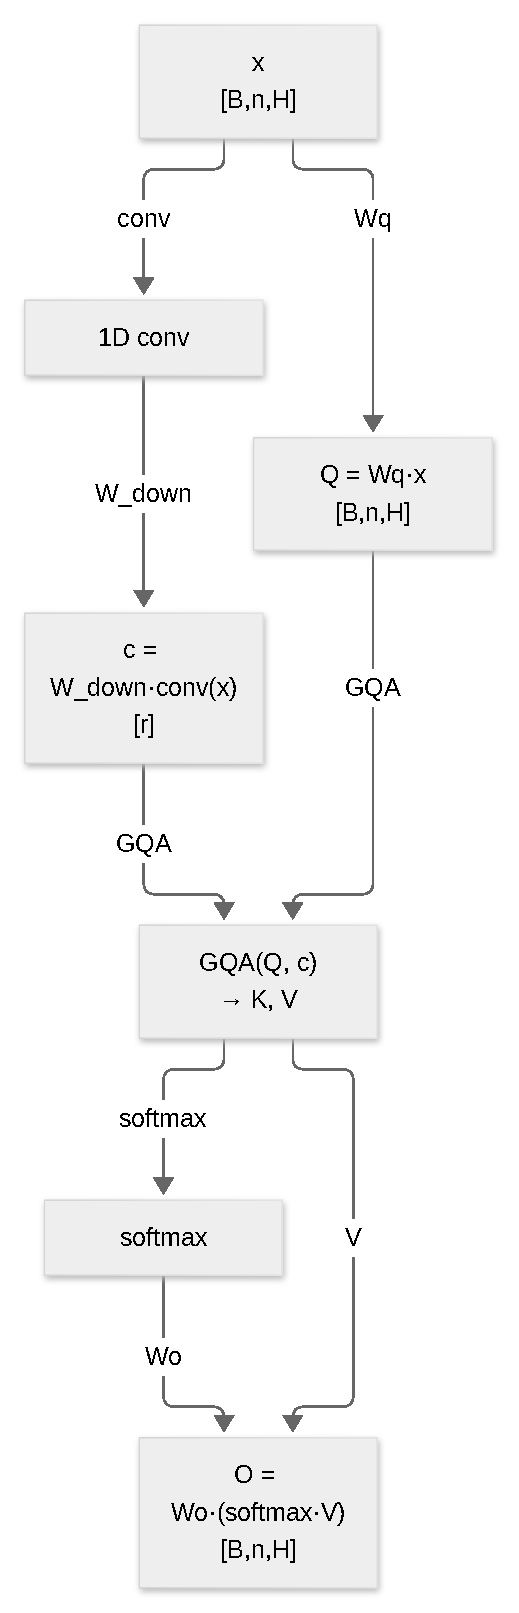
\includegraphics{figures/mixers/ccgqa.pdf}}
\caption{Dataflow of compressed convolutional grouped-query attention: the convolution latent supplies a grouped-query key/value expansion.}
\label{fig:mixer-ccgqa}
\end{figure}
Compressed Convolutional Grouped Query Attention (CCGQA) \citep{figliola_cca_2025} extends CCA with GQA-style key/value head sharing applied \emph{inside} the compressed latent, and \textbf{decouples} the query and KV compression rates: queries are compressed by $C_1$ and keys/values by $C_2 \geq C_1$. The per-head latent dimension $d_h$ must match between query and key heads, enforcing the constraint $C_2 / C_1 = n_h / n_{kv}$. KV heads are shared per group (replicated to match query heads), and the qk-mean bias uses broadcast/reduce operators $B_{\text{group}}$ (replicate KV heads to query heads) and $E_{\text{group}}$ (average query heads within each group). CCGQA achieves the best reported loss at 8$\times$ KV-cache compression with no quality drop versus MHA.

\subsubsection{Mathematical Formulation}
Same pipeline as CCA, with decoupled latents:
\[
\tilde{q}_{\text{pre}} = \tilde{W}_Q\, x \in \mathbb{R}^{E/C_1}, \qquad
\tilde{k}_{\text{pre}} = \tilde{W}_K\, x \in \mathbb{R}^{E/C_2}, \qquad C_2 \geq C_1.
\]
\[
\text{qk\_mean}_q = \tfrac{1}{2}(\tilde{q}_{\text{pre}} + B_{\text{group}}(\tilde{k}_{\text{pre}})), \qquad
\text{qk\_mean}_k = E_{\text{group}}(\text{qk\_mean}_q).
\]
\[
\text{attn} = \texttt{softmax}\!\left(\frac{\text{RoPE}(\hat{q})\, \text{RoPE}(\hat{k})^\top}{\sqrt{d_h}}\right) \tilde{v}, \qquad
\mathbf{Y} = \tilde{W}_O\, \text{attn}.
\]

\subsubsection{Key Characteristics}
\begin{itemize}[leftmargin=*]
    \item \textbf{Training complexity}: $\mathcal{O}(n^2 \cdot d / C_1)$ ($S^2$ term scales by $1/C_1$; projection terms by $1/C_1 + 1/C_2$).
    \item \textbf{Inference complexity}: $\mathcal{O}(n)$ per token, $\mathcal{O}(\tilde{e}_{kv} \cdot n)$ KV-cache space ($C_2$-compressed, group-shared).
    \item \textbf{Trainable}: $C_1$, $C_2$, $n_{kv}$, and all CCA tricks are configurable. Constraint: $C_2/C_1 = n_h/n_{kv}$.
    \item \textbf{Strengths}: Decoupled compression enables smooth Pareto frontier; same arithmetic intensity as GQA; best loss at 8$\times$ cache reduction.
    \item \textbf{Limitations}: Same quadratic $S^2$ (only reduced by $C_1$); fused kernel needed; two value projections add complexity.
\end{itemize}

The latent family shows a clear progression along two axes: (i) \textbf{rank compression}, moving from full heads (MHA) to a shared latent (MLA) to partitioned sub-head latents (MLRA), and (ii) \textbf{deployment adaptivity}, moving from a single decode path to hardware-adaptive dispatch (GQLA) and temporal cache merging (MTLA). Tucker Attention provides the unifying algebraic frame: MHA, GQA, and MLA are all special cases of a Tucker factorisation with appropriate rank choices. CCA and CCGQA take a fundamentally different approach: rather than compressing the KV-cache and then up-projecting for full-width attention (MLA/GQLA/MLRA), they perform attention \emph{entirely inside} the compressed latent space, reducing not just the cache but also the attention FLOPs by the compression factor. CCGQA further decouples query and KV compression rates, achieving the best reported loss at 8$\times$ KV-cache compression. Gaussian Mixture Attention (GMA) changes the routing philosophy entirely: instead of a low-rank linear bottleneck, it routes through $K$ learned probabilistic Gaussian components, achieving linear-time $\mathcal{O}(NK)$ sequence mixing for fixed $K$ while retaining a normalised attention-style interpretation.

\subsection{Gaussian Mixture Attention (GMA)}

\begin{figure}[H]
\centering
\fitfigure{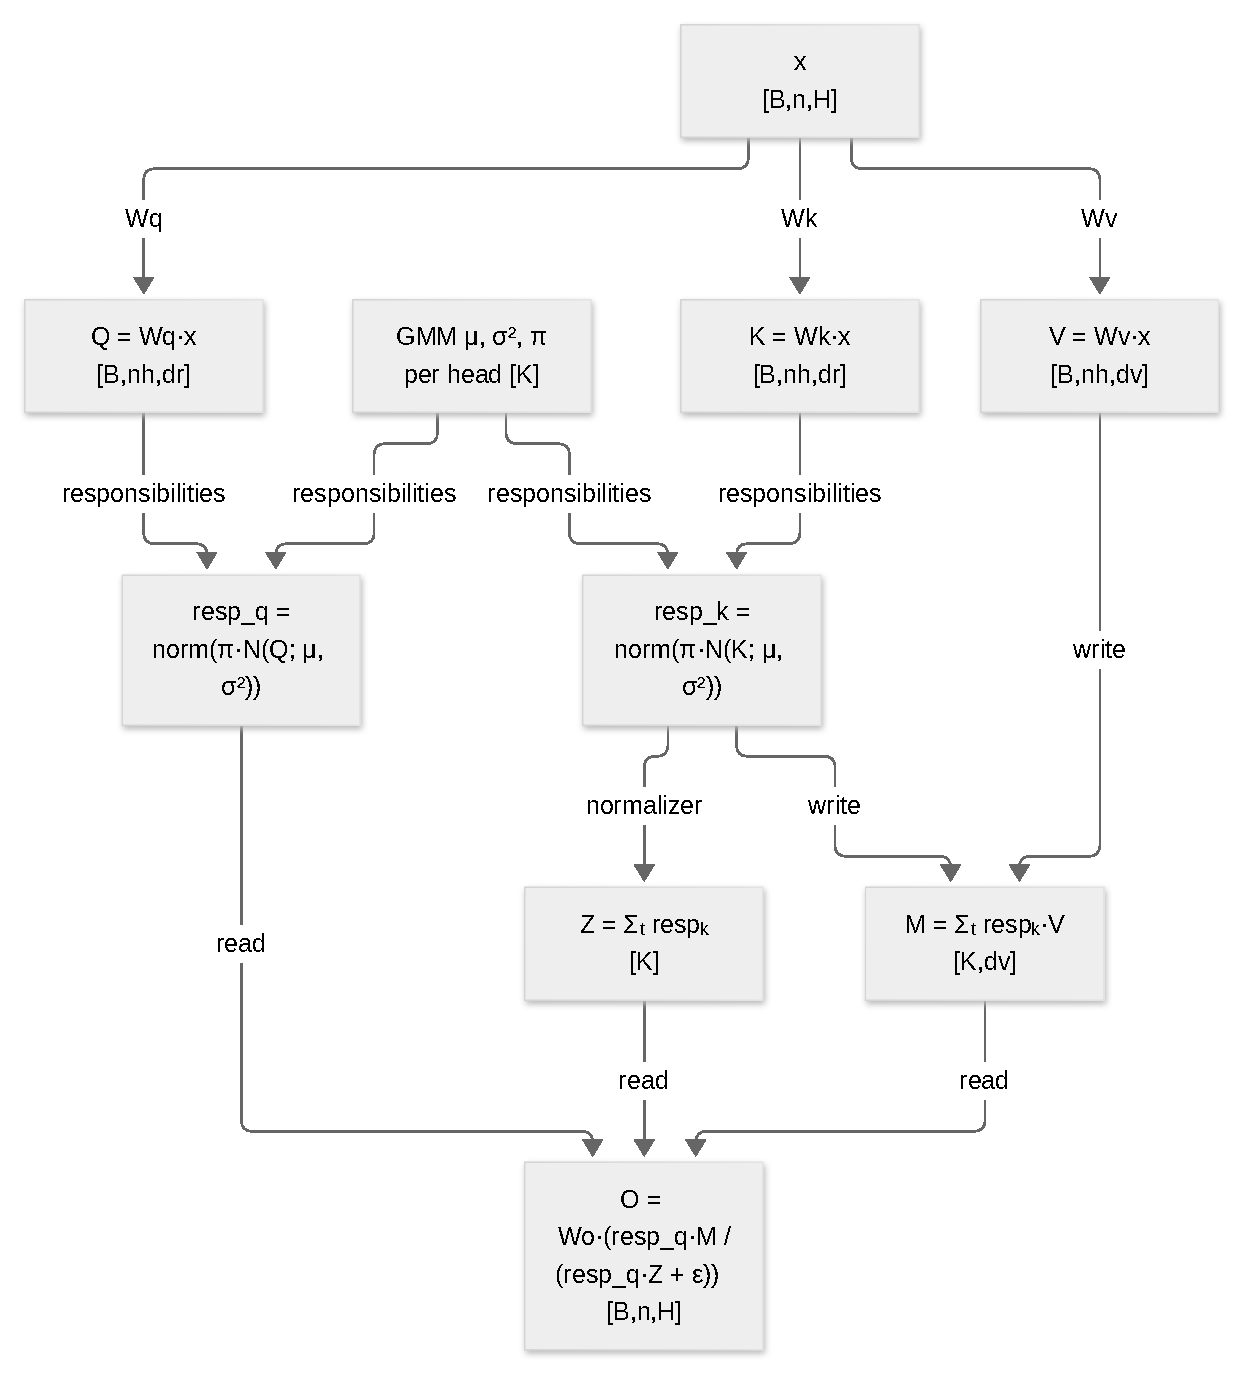
\includegraphics{figures/mixers/gma.pdf}}
\caption{Dataflow of Gaussian-mixture attention: per-head Gaussian responsibilities route keys and values into a $K$-slot memory that the query reads back, normalized by $Z$.}
\label{fig:mixer-gma}
\end{figure}
Gaussian Mixture Attention (GMA) \citep{huang_gma_2026} replaces the explicit pairwise $QK^\top$ interaction of standard dot-product attention with probabilistic routing through $K$ learned Gaussian-mixture components per head. Queries and keys are mapped to posterior \emph{responsibility} vectors over a shared latent routing space; their overlap defines an implicit responsibility-space affinity, while values are written into and read from a $K$-slot latent memory. By exploiting the associativity of matrix multiplication, GMA avoids materialising the induced $N \times N$ affinity matrix and instead uses two $N \times K$ responsibility matrices whose dominant activation storage scales as $\mathcal{O}(NK)$ rather than $\mathcal{O}(N^2)$ for fixed $K$. The Gaussian mixture parameters---component means $\mu$, diagonal covariances (reparameterised via $\sigma^2 = \text{softplus}(\omega) + \epsilon_\sigma$) and mixture-prior logits $\alpha$ (with $\pi = \text{softmax}(\alpha)$)---are fully differentiable learnable parameters optimised by standard backpropagation, with no EM loop or auxiliary clustering loss.

\subsubsection{Mathematical Formulation}
Per head, with routing dimension $d_r$ and value dimension $d_v$:
\[
Q_X = X W_Q \in \mathbb{R}^{N \times d_r}, \quad
K_X = X W_K \in \mathbb{R}^{N \times d_r}, \quad
V_X = X W_V \in \mathbb{R}^{N \times d_v}.
\]
The posterior responsibility of component $k$ for a routing vector $x_i$ is
\[
\gamma_{i,k} = p(z{=}k \mid x_i) = \frac{\pi_k\, \mathcal{N}(x_i \mid \mu_k, \Sigma_k)}{\sum_{\ell=1}^{K} \pi_\ell\, \mathcal{N}(x_i \mid \mu_\ell, \Sigma_\ell)},
\qquad \Sigma_k = \mathrm{diag}(\sigma_{k,1}^2, \dots, \sigma_{k,d_r}^2),
\]
yielding responsibility matrices $\Gamma^Q, \Gamma^K \in \mathbb{R}^{N \times K}$. The bidirectional output is computed by the associative write--read pair
\[
\tilde V = (\Gamma^K)^\top V_X \in \mathbb{R}^{K \times d_v}, \qquad
Z = (\Gamma^K)^\top \mathbf{1}_N \in \mathbb{R}^{K}, \qquad
O = \frac{\Gamma^Q \tilde V}{\Gamma^Q Z + \epsilon},
\]
which never materialises the implicit normalised affinity $A^{\text{GMA}}_{ij} = \frac{\sum_k \gamma^Q_{i,k} \gamma^K_{j,k}}{\sum_\ell \sum_k \gamma^Q_{i,k} \gamma^K_{\ell,k} + \epsilon}$. For autoregressive modelling the global write statistics are replaced by prefix-restricted cumulative sums $\tilde V^{(i)}_k = \sum_{j \le i} \gamma^K_{j,k} V_{X,j}$ and $Z^{(i)}_k = \sum_{j \le i} \gamma^K_{j,k}$, enforcing causality while preserving the fixed-$K$ linear scaling.

\subsubsection{Algorithmic Pseudocode}
\begin{algorithmic}[1]
\State \textbf{Input:} hidden state $X \in \mathbb{R}^{N \times d}$, $K$ components, routing dim $d_r$, value dim $d_v$, params $\{\mu_k, \omega_k, \alpha_k\}_{k=1}^{K}$
\State $Q_X \gets X W_Q$, \quad $K_X \gets X W_K$, \quad $V_X \gets X W_V$ \Comment{head projections}
\State $\sigma^2_k \gets \text{softplus}(\omega_k) + \epsilon_\sigma$, \quad $\pi_k \gets \text{softmax}(\alpha)_k$ \Comment{reparameterise}
\State $\Gamma^Q \gets \texttt{softmax}_k\!\left(\log \pi_k - \tfrac{d_r}{2}\log 2\pi - \tfrac{1}{2}\sum_m \log \sigma^2_{k,m} - \tfrac{1}{2}\sum_m \frac{(q_{i,m}-\mu_{k,m})^2}{\sigma^2_{k,m}}\right)$
\State $\Gamma^K \gets$ same as $\Gamma^Q$ applied to $K_X$
\If{causal}
    \State $\tilde V \gets \texttt{cumsum}_n(\Gamma^K \otimes V_X)$, \quad $Z \gets \texttt{cumsum}_n(\Gamma^K)$ \Comment{prefix-restricted}
\Else
    \State $\tilde V \gets (\Gamma^K)^\top V_X$, \quad $Z \gets (\Gamma^K)^\top \mathbf{1}_N$ \Comment{global write}
\EndIf
\State $O \gets \Gamma^Q \tilde V \,/\, (\Gamma^Q Z + \epsilon)$ \Comment{normalised read}
\State \textbf{Output:} $\mathbf{Y} = O W_O$
\end{algorithmic}

\subsubsection{Key Characteristics}
\begin{itemize}[leftmargin=*]
    \item \textbf{Training complexity}: $\mathcal{O}(N K d_r + N K d_v)$ for fixed $K$, linear in the sequence length $N$.
    \item \textbf{Inference complexity}: $\mathcal{O}(K)$ per token (responsibilities + latent read), $\mathcal{O}(NK)$ activation storage.
    \item \textbf{Trainable}: fully differentiable GMM parameters $\{\mu, \omega, \alpha\}$ per head, optimised end-to-end without EM.
    \item \textbf{Strengths}: Fixed-$K$ linear-time sequence mixing; probabilistic interpretable routing; bidirectional and causal variants; non-negative low-rank affinity interpretation $A^{\text{GMA}} = \mathrm{diag}(d)^{-1} \Gamma^Q (\Gamma^K)^\top$.
    \item \textbf{Limitations}: Quality depends on $K$ and the routing dimension $d_r$; causal GMA trails optimised SDPA and state-space models on WikiText-103 in the paper's current implementation; not a universal replacement for softmax attention.
\end{itemize}
\subsection{Kronecker Product Attention (KPA)}
\label{sec:kpa}

\begin{figure}[t]
\centering
\fitfigure{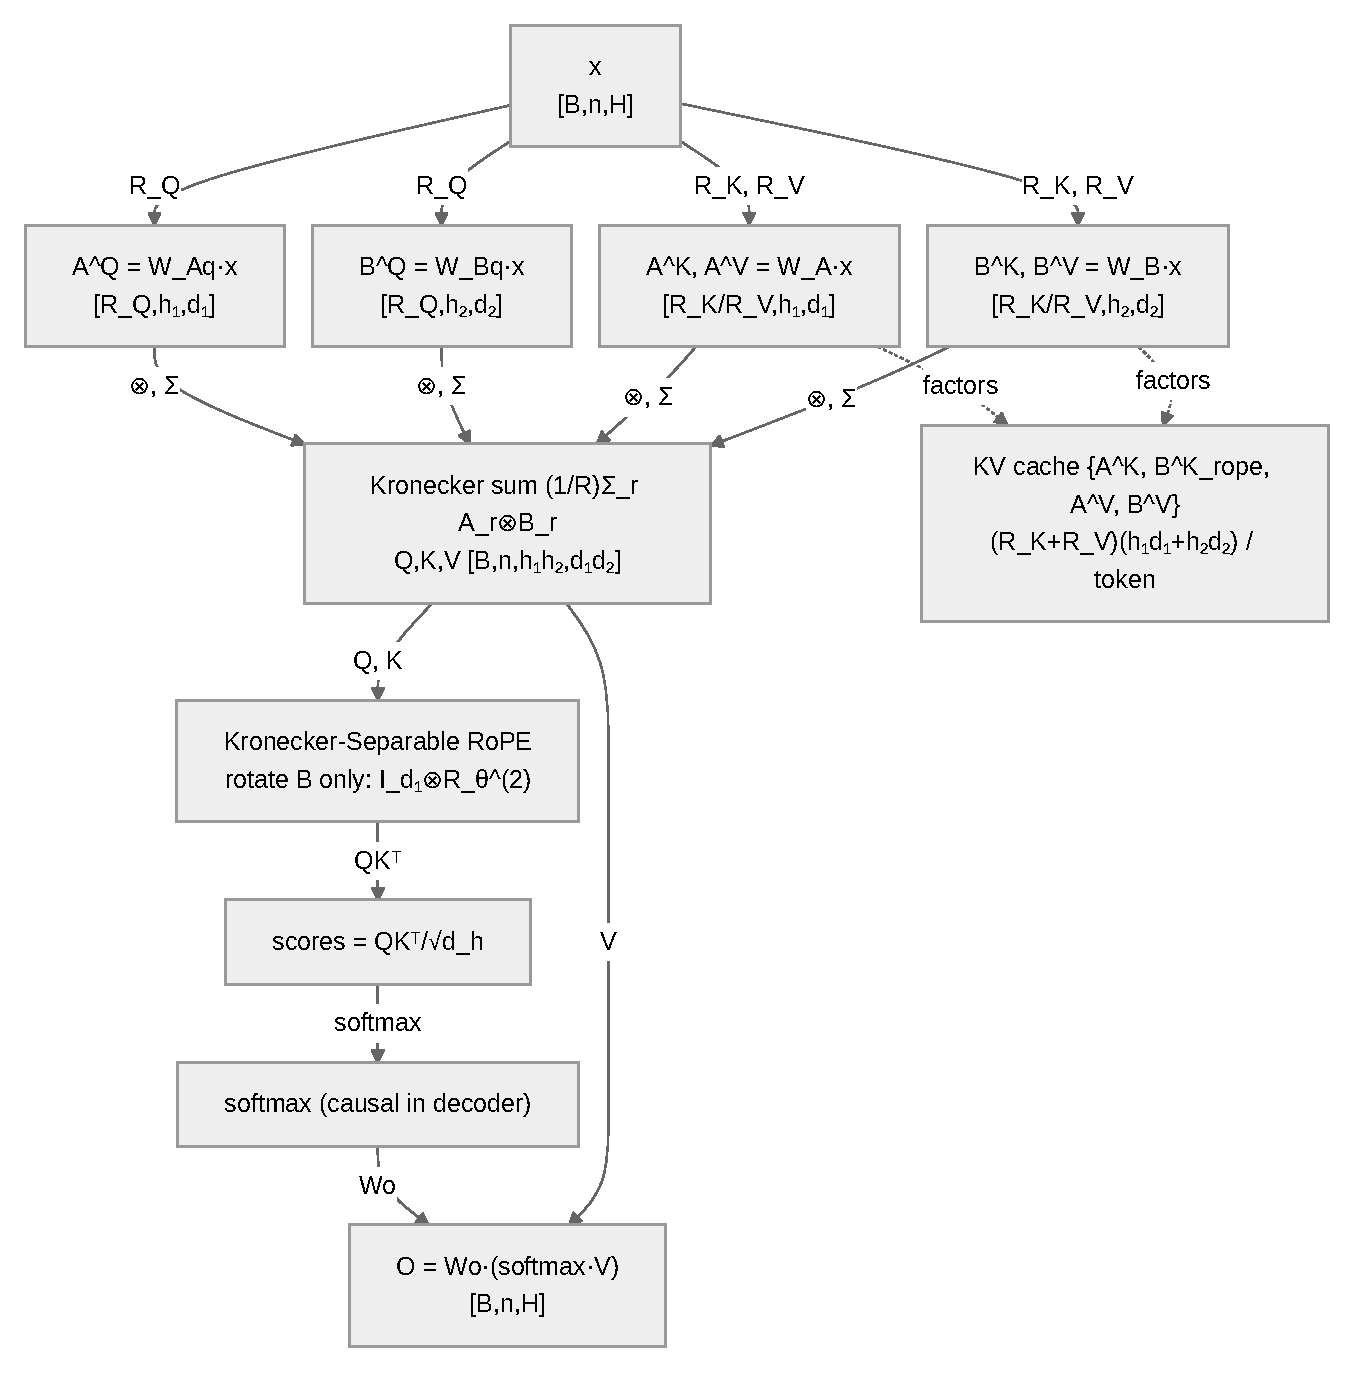
\includegraphics{figures/mixers/kpa.pdf}}
\caption{Kronecker Product Attention (KPA). Each per-token query, key and value matrix is a normalized sum of Kronecker products of two compact contextual factors: $A_r\in\mathbb{R}^{h_1\times d_1}$ partitions the head axis, $B_r\in\mathbb{R}^{h_2\times d_2}$ the within-head feature axis. Only the K/V factors enter the cache, and Kronecker-Separable RoPE rotates the $B$ factor alone.}
\label{fig:mixer-kpa}
\end{figure}

Kronecker Product Attention (KPA) \citep{nikpour_kpa_2026} is a KV-compression mixer that factorises the per-token key, value and query matrices as normalized sums of Kronecker products of compact contextual factors. Unlike Tensor Product Attention (TPA), whose CP decomposition operates on vectors, KPA acts on matrices and therefore encodes structure at both the head and the feature level; rank-one CP factorisation is recovered as the degenerate split $h_1=h, d_1=1, h_2=1, d_2=d_h$, so KPA strictly generalises TPA at the same parameter budget.

\subsubsection{Mathematical Foundation}
Let $h = h_1 h_2$ be the number of heads and $d_h = d_1 d_2$ the head width. For a token with hidden state $x_t \in \mathbb{R}^{d_{\text{model}}}$, the Kronecker product obeys the mixed-product identity
\[
(M \otimes N)(P \otimes Q) = (MP) \otimes (NQ),
\]
and the three projections are
\[
Q_t = \frac{1}{R_Q}\sum_{r=1}^{R_Q} A^Q_r(x_t)\otimes B^Q_r(x_t),\quad
K_t = \frac{1}{R_K}\sum_{r=1}^{R_K} A^K_r(x_t)\otimes B^K_r(x_t),\quad
V_t = \frac{1}{R_V}\sum_{r=1}^{R_V} A^V_r(x_t)\otimes B^V_r(x_t),
\]
with $A^\cdot_r(x_t) = W^{A^\cdot}_r x_t \in \mathbb{R}^{h_1\times d_1}$ and $B^\cdot_r(x_t) = W^{B^\cdot}_r x_t \in \mathbb{R}^{h_2\times d_2}$ produced by independent bias-free linear maps; the rank index is merged into a single batched projection per factor kind. Heads are indexed by pairs $(i_1,i_2)$ with $i_1\in[h_1]$, $i_2\in[h_2]$, and the mixed-product identity factorises every attention score into a head-level and a feature-level inner product:
\[
\mathrm{score}_{(i_1,i_2)}(t,s) = \frac{1}{R_Q R_K}\sum_{r=1}^{R_Q}\sum_{r'=1}^{R_K}
\bigl[(A^Q_r)_{i_1}^{\top}(A^K_{r'})_{i_1}\bigr]\,
\bigl[(B^Q_r)_{i_2}^{\top}(B^K_{r'})_{i_2}\bigr].
\]
Kronecker-Separable RoPE uses the operator $R_{\mathrm{KPA}}(t) = I_{d_1}\otimes R^{(2)}_\theta(t)$ with frequencies $\theta_j = 10000^{-2j/d_2}$ calibrated to $d_2$. Because $(I_{d_1}\otimes R^{(2)}_\theta(t))((A_r)_{i_1}\otimes(B_r)_{i_2}) = (A_r)_{i_1}\otimes R^{(2)}_\theta(t)(B_r)_{i_2}$, only the $B$ factor is rotated, the $A$ factor is cached unrotated, and the relative-position property follows from $R^{(2)}_\theta(t)^{\top}R^{(2)}_\theta(s) = R^{(2)}_\theta(s-t)$; no decoupled RoPE branch is needed.
The cache stores $\{A^K_r, B^K_r\}_{r=1}^{R_K}\cup\{A^V_r, B^V_r\}_{r=1}^{R_V}$ per token (with $B^K$ pre-rotated), at a cost of $(R_K+R_V)(h_1d_1+h_2d_2)$ floats instead of $2h_1h_2d_1d_2$ for MHA, i.e. a compression factor
\[
C_{\mathrm{KPA}} = \frac{2h_1h_2d_1d_2}{(R_K+R_V)(h_1d_1+h_2d_2)},
\]
which increases with factor asymmetry.

\subsubsection{Algorithmic Pseudocode}
\begin{algorithmic}[1]
\State \textbf{Input:} hidden state $X\in\mathbb{R}^{n\times d}$, splits $h_1 h_2 = H$, $d_1 d_2 = d_h$, ranks $R_Q, R_K, R_V$
\State $A^Q \gets \texttt{reshape}(X W^{A^Q}, n, R_Q, h_1, d_1)$, \quad $B^Q \gets \texttt{reshape}(X W^{B^Q}, n, R_Q, h_2, d_2)$
\State likewise $(A^K,B^K)$ with $R_K$ and $(A^V,B^V)$ with $R_V$ \Comment{bias-free factor projections}
\For{each of $Q,K,V$}
    \State $M \gets \frac{1}{R}\sum_{r} A_r \otimes B_r$ \Comment{Kronecker sum, eqs. (2)--(4)}
    \State $M \gets \texttt{reshape}(M, n, h_1 h_2, d_1 d_2)$ \Comment{head $(i_1,i_2)\mapsto i_1 h_2 + i_2$}
\EndFor
\State apply $R_{\mathrm{KPA}}$ to $Q$ and $K$ \Comment{rotate $B$ only; $A$ stays unrotated}
\State $S \gets QK^{\top}/\sqrt{d_h}$; \quad $S \gets \texttt{mask}(S)$ if causal
\State $O \gets \texttt{softmax}(S)\,V$; \quad \textbf{Output:} $Y = O W_O$
\end{algorithmic}

\subsubsection{Key Characteristics}
\begin{itemize}[leftmargin=*]
    \item \textbf{Training complexity}: $\mathcal{O}(n^2 d)$ attention plus $\mathcal{O}\big(n\,d\,(R_Q+R_K+R_V)(h_1d_1+h_2d_2)\big)$ factor projections.
    \item \textbf{Inference complexity}: $\mathcal{O}(n\,h\,d_h)$ attention per step and $\mathcal{O}\big((R_K+R_V)(h_1d_1+h_2d_2)\big)$ cached state per token; $6.4\times$--$10\times$ KV compression in the paper.
    \item \textbf{Trainable}: trained from scratch (nanoGPT + SwiGLU + RoPE) at 125M, 353M, 773M and 1.5B parameters on FineWeb-Edu for $\sim$50B tokens.
    \item \textbf{Strengths}: strict generalisation of TPA with richer block structure at matched parameters; RoPE-compatible without MLA's decoupled branch; the head split $h_1\times h_2$ is a design-time compression/accuracy knob with no architectural change.
    \item \textbf{Limitations}: the paper fixes $d_1=d_2=8$ and evaluates only causal language models; an efficient factored decoding kernel and long-context evaluation are left as future work; materialising the Kronecker sums is quadratic in the sequence length like dense attention.
\end{itemize}

\subsection{Tensor Product Attention (TPA)}
\label{sec:tpa}

\begin{figure}[t]
\centering
\fitfigure{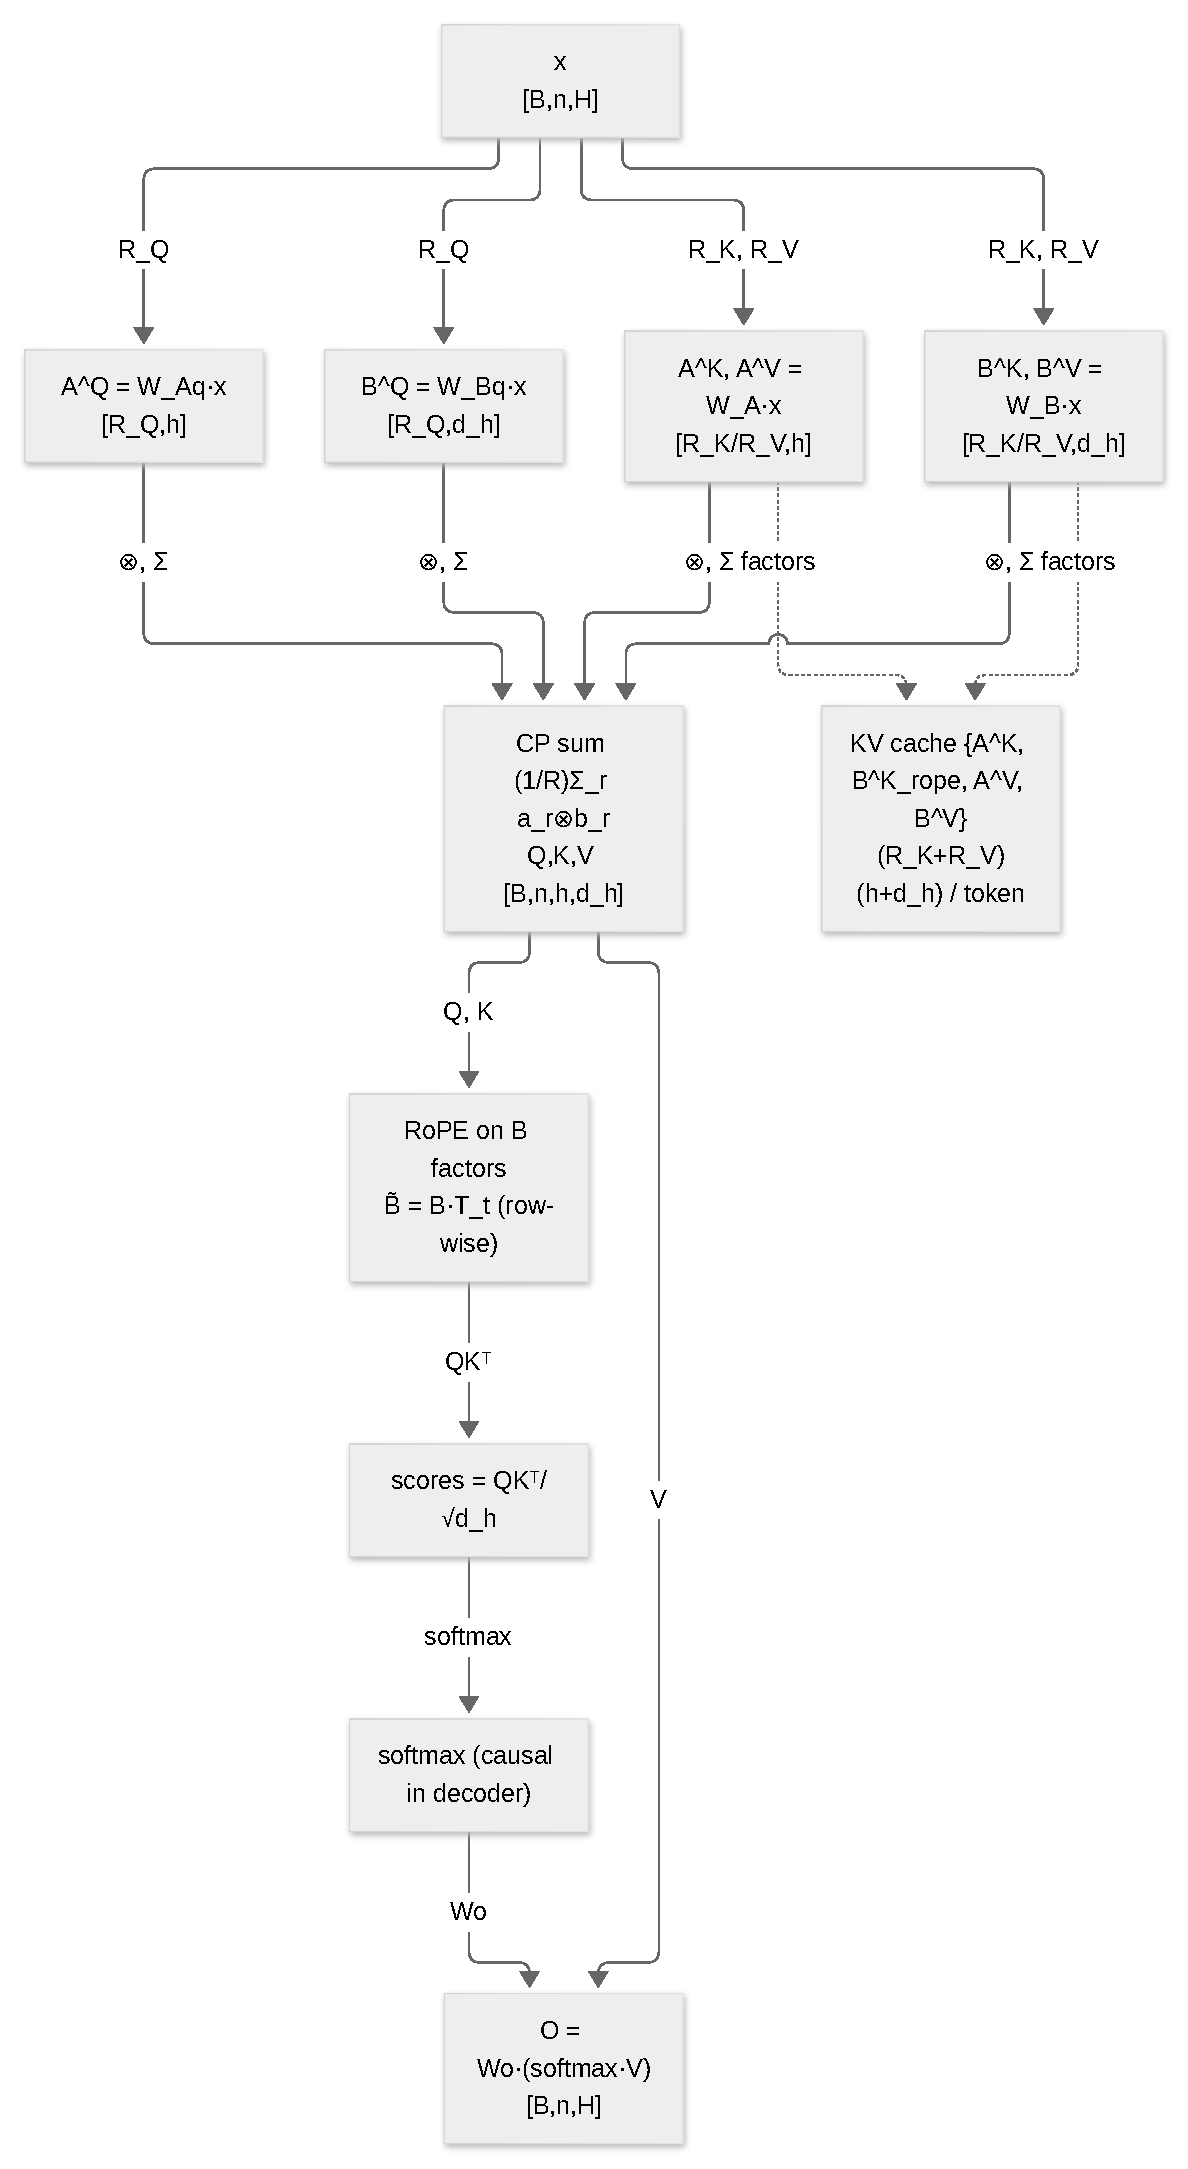
\includegraphics{figures/mixers/tpa.pdf}}
\caption{Tensor Product Attention (TPA). Each per-token query, key and value slice is a normalized CP sum $\frac{1}{R}\sum_r a_r(x_t)\otimes b_r(x_t)$ of a head-axis vector $a_r\in\mathbb{R}^{h}$ and a feature-axis vector $b_r\in\mathbb{R}^{d_h}$. RoPE acts row-wise on the $B$ factors, so cached keys can be stored pre-rotated; only the four factor streams enter the cache.}
\label{fig:mixer-tpa}
\end{figure}

Tensor Product Attention (TPA) \citep{zhang_tpa_2025} is the canonical activation-space tensor decomposition for attention: rather than factorising the projection weights (as Tucker Attention does), it factorises the per-token query, key and value activations themselves into rank-one outer products of contextual vectors. It is the vector (CP) special case of KPA \citep{nikpour_kpa_2026}, recovered at $h_1=h$, $d_1=1$, $h_2=1$, $d_2=d_h$.

\subsubsection{Mathematical Foundation}
With $h$ heads, head width $d_h$ and CP ranks $R_Q,R_K,R_V$, each token's slice is
\[
Q_t = \frac{1}{R_Q}\sum_{r=1}^{R_Q} a^Q_r(x_t)\otimes b^Q_r(x_t),\quad
K_t = \frac{1}{R_K}\sum_{r=1}^{R_K} a^K_r(x_t)\otimes b^K_r(x_t),\quad
V_t = \frac{1}{R_V}\sum_{r=1}^{R_V} a^V_r(x_t)\otimes b^V_r(x_t),
\]
with $a^\cdot_r(x_t)=W^{a^\cdot}_r x_t\in\mathbb{R}^{h}$ and $b^\cdot_r(x_t)=W^{b^\cdot}_r x_t\in\mathbb{R}^{d_h}$ produced by bias-free linear maps. Merging the rank index into one projection per factor side, $a_Q(x_t)=W^{aQ}x_t\in\mathbb{R}^{R_Q h}$ and $b_Q(x_t)=W^{bQ}x_t\in\mathbb{R}^{R_Q d_h}$, and reshaping into $A_Q(x_t)\in\mathbb{R}^{R_Q\times h}$, $B_Q(x_t)\in\mathbb{R}^{R_Q\times d_h}$ gives the compact form
\[
Q_t = \frac{1}{R_Q}A_Q(x_t)^{\top}B_Q(x_t)\in\mathbb{R}^{h\times d_h},
\]
and attention is the ordinary scaled dot-product map
\[
\mathrm{head}_i = \mathrm{Softmax}\!\left(\frac{Q_iK_i^{\top}}{\sqrt{d_h}}\right)V_i,\qquad
\mathrm{TPA}(Q,K,V)=\mathrm{Concat}(\mathrm{head}_1,\dots,\mathrm{head}_h)\,W^O .
\]
Because RoPE rotates only the head-width axis it commutes with the factorisation (Theorem~3.1 of the paper): $B^\cdot(x_t)\mapsto B^\cdot(x_t)T_t$ row-wise and $\widetilde{Q}_t=Q_tT_t=\frac{1}{R_Q}A_Q(x_t)^{\top}\widetilde{B}_Q(x_t)$, preserving the relative-position identity $\widetilde{Q}_t\widetilde{K}_s^{\top}=Q_tT_{t-s}K_s^{\top}$. The cache holds $\{A^K,\widetilde{B}^K,A^V,B^V\}$ per token, i.e.
\[
\mathrm{KV}_{\mathrm{TPA}}=(R_K+R_V)(h+d_h)\ \text{floats/token}
\quad\text{vs.}\quad 2hd_h\ \text{for MHA},
\]
and the attention-layer parameter count (Table~1 of the paper) is
\[
P_{\mathrm{TPA}} = d_{\text{model}}\,(R_Q+R_K+R_V)(h+d_h) + d_{\text{model}}\,h\,d_h .
\]

\subsubsection{Algorithmic Pseudocode}
\begin{algorithmic}[1]
\State \textbf{Input:} hidden state $X\in\mathbb{R}^{n\times d}$, $h$ heads, head width $d_h$, ranks $R_Q,R_K,R_V$
\State $A^Q\gets\texttt{reshape}(XW^{aQ}, n, R_Q, h)$, \quad $B^Q\gets\texttt{reshape}(XW^{bQ}, n, R_Q, d_h)$
\State likewise $(A^K,B^K)$ with $R_K$ and $(A^V,B^V)$ with $R_V$ \Comment{bias-free factor projections}
\For{each of $Q,K,V$}
    \State $M\gets \frac{1}{R}\sum_{r} a_r\otimes b_r = \frac{1}{R}A^{\top}B$ \Comment{CP sum, eq.~(3.1)}
\EndFor
\State apply RoPE to $B^Q$ and $B^K$ row-wise \Comment{pre-rotation, eq.~(3.5); current-step only at decode}
\State $S\gets QK^{\top}/\sqrt{d_h}$; \quad $S\gets\texttt{mask}(S)$ if causal
\State $O\gets\texttt{softmax}(S)V$; \quad \textbf{Output:} $Y=OW_O$
\end{algorithmic}
A fused factor-space variant (FlashTPA, Appendix~A of the paper) computes the head-shared feature dots $P[b,q,k,r,s]=\langle B^Q_{q,r},B^K_{k,s}\rangle$ first, mixes them with $A^Q,A^K$ into the logits, and aggregates values through $A^V,B^V$ without ever materialising $Q,K,V$; it reduces FLOPs whenever $R_QR_KD + hR_QR_K + hR_VE < 2hd_h$. This implementation uses the materialised path and keeps the factor-space variant as a kernel-level optimisation.

\subsubsection{Key Characteristics}
\begin{itemize}[leftmargin=*]
    \item \textbf{Training complexity}: $\mathcal{O}(n^2 d)$ attention plus $\mathcal{O}\big(n\,d\,(R_Q+R_K+R_V)(h+d_h)\big)$ factor projections; the specialised path is $\mathcal{O}(n^2R_QR_Kd_h + n^2hR_QR_K + n^2hR_Vd_h)$.
    \item \textbf{Inference complexity}: $\mathcal{O}(M R_QR_Kd_h + MhR_QR_K + MhR_Vd_h)$ per decode step against a cache of length $M$; $(R_K+R_V)(h+d_h)$ cached floats per token, an order of magnitude below MHA at $R_K,R_V\le 2$.
    \item \textbf{Trainable}: trained from scratch; T6 composes TPA with RMSNorm and SwiGLU blocks and is pretrained with next-token prediction.
    \item \textbf{Strengths}: native RoPE (and generic position-encoding) compatibility without MLA's decoupled branch; better validation perplexity and downstream scores than MHA, MQA, GQA and MLA at matched parameter counts; MHA/MQA/GQA are recovered as non-contextual rank-$h$/rank-1/rank-$G$ special cases, which makes the rank a single design knob.
    \item \textbf{Limitations}: extra rank hyperparameters ($R_Q,R_K,R_V$) and a factorisation cost on the materialised path; quality depends on rank choice; the paper evaluates causal language models only; the full speed-up requires the FlashTPA kernel.
\end{itemize}
